\documentclass[tikz,border=10pt]{standalone}
\usepackage{amsmath}
\usetikzlibrary{arrows.meta, positioning, calc, decorations.pathreplacing}
\definecolor{c1}{HTML}{000000}
\definecolor{c2}{HTML}{233D4D}
\definecolor{c3}{HTML}{FE7F2D}
\definecolor{c4}{HTML}{EAECF0}
\definecolor{labelcolor}{HTML}{5F6B75}
\begin{document}
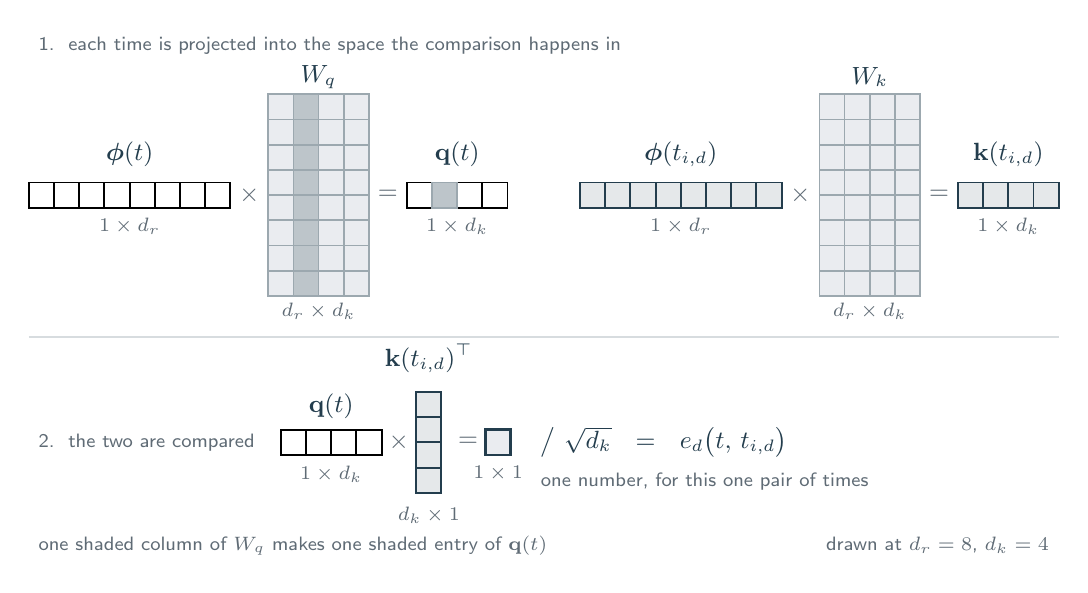
\begin{tikzpicture}[
    every node/.style={font=\sffamily},
    lab/.style={font=\sffamily\scriptsize, text=labelcolor},
    tag/.style={font=\sffamily\small, text=c2},
    op/.style={font=\sffamily\small, text=labelcolor},
    qc/.style={draw=c1, fill=white, line width=0.7pt},
    kc/.style={draw=c2, fill=c2!12, line width=0.7pt},
    wc/.style={draw=c2!45, fill=c4, line width=0.6pt},
    hc/.style={draw=c2!45, fill=c2!30, line width=0.6pt},
    ec/.style={draw=c2, fill=c4, line width=1.0pt},
]
\def\cs{0.32}

% ---- a 1 x n row of cells, style #1, from (#2,#3), n = #4
\newcommand{\rowvec}[4]{%
  \foreach \i in {0,...,\the\numexpr#4-1\relax}{%
    \draw[#1] ({#2+\i*\cs}, #3) rectangle ({#2+\i*\cs+\cs}, {#3+\cs});}}
% ---- an r x c block, style #1, top-left (#2,#3), rows #4, cols #5
\newcommand{\blockmat}[5]{%
  \foreach \r in {0,...,\the\numexpr#4-1\relax}{%
    \foreach \c in {0,...,\the\numexpr#5-1\relax}{%
      \draw[#1] ({#2+\c*\cs}, {#3-\r*\cs-\cs}) rectangle ({#2+\c*\cs+\cs}, {#3-\r*\cs});}}}

\node[lab, anchor=west] at (0.40, 6.30)
     {1.\ \ each time is projected into the space the comparison happens in};

% ============================================================ query group
\rowvec{qc}{0.40}{4.24}{8}
\node[tag]  at (1.68, 4.92) {$\boldsymbol{\phi}(t)$};
\node[lab]  at (1.68, 4.00) {$1 \times d_r$};

\node[op] at (3.20, 4.40) {$\times$};

\blockmat{wc}{3.44}{5.68}{8}{4}
\foreach \r in {0,...,7}{
  \draw[hc] ({3.44+1*\cs}, {5.68-\r*\cs-\cs}) rectangle ({3.44+2*\cs}, {5.68-\r*\cs});}
\node[tag] at (4.08, 5.90) {$W_q$};
\node[lab] at (4.08, 2.92) {$d_r \times d_k$};

\node[op] at (4.96, 4.40) {$=$};

\rowvec{qc}{5.20}{4.24}{4}
\draw[hc] ({5.20+1*\cs}, 4.24) rectangle ({5.20+2*\cs}, 4.56);
\node[tag] at (5.84, 4.92) {$\mathbf{q}(t)$};
\node[lab] at (5.84, 4.00) {$1 \times d_k$};

% ============================================================== key group
\rowvec{kc}{7.40}{4.24}{8}
\node[tag]  at (8.68, 4.92) {$\boldsymbol{\phi}(t_{i,d})$};
\node[lab]  at (8.68, 4.00) {$1 \times d_r$};

\node[op] at (10.20, 4.40) {$\times$};

\blockmat{wc}{10.44}{5.68}{8}{4}
\node[tag] at (11.08, 5.90) {$W_k$};
\node[lab] at (11.08, 2.92) {$d_r \times d_k$};

\node[op] at (11.96, 4.40) {$=$};

\rowvec{kc}{12.20}{4.24}{4}
\node[tag] at (12.84, 4.92) {$\mathbf{k}(t_{i,d})$};
\node[lab] at (12.84, 4.00) {$1 \times d_k$};

\draw[c2!18, line width=0.8pt] (0.40, 2.60) -- (13.48, 2.60);

% ================================================== the comparison itself
\node[lab, anchor=west] at (0.40, 1.26) {2.\ \ the two are compared};

\rowvec{qc}{3.60}{1.10}{4}
\node[tag] at (4.24, 1.72) {$\mathbf{q}(t)$};
\node[lab] at (4.24, 0.86) {$1 \times d_k$};

\node[op] at (5.10, 1.26) {$\times$};

\blockmat{kc}{5.32}{1.90}{4}{1}
\node[tag, anchor=south] at (5.48, 2.02) {$\mathbf{k}(t_{i,d})^{\top}$};
\node[lab, anchor=north] at (5.48, 0.56) {$d_k \times 1$};

\node[op] at (5.98, 1.26) {$=$};

\draw[ec] (6.20, 1.10) rectangle (6.52, 1.42);
\node[lab] at (6.36, 0.86) {$1 \times 1$};

\node[tag, anchor=west] at (6.78, 1.26)
     {$\big/\ \sqrt{d_k}\ \ =\ \ e_d\big(t,\, t_{i,d}\big)$};
\node[lab, anchor=west] at (6.78, 0.76)
     {one number, for this one pair of times};

\node[lab, anchor=west] at (0.40, -0.05)
     {one shaded column of $W_q$ makes one shaded entry of $\mathbf{q}(t)$};
\node[lab, anchor=east] at (13.48, -0.05) {drawn at $d_r = 8$, $d_k = 4$};
\end{tikzpicture}
\end{document}
